\documentclass{article}
\usepackage{tikz}
\usepackage{circuitikz}
\usepackage{pdflscape}
\usepackage[margin=2cm]{geometry}
\usepackage{caption}
\usepackage{multirow}
\usepackage{makecell}

\usetikzlibrary{shapes,arrows,positioning,fit}

\begin{document}

\begin{landscape}
\section*{General Overview Block Diagram}
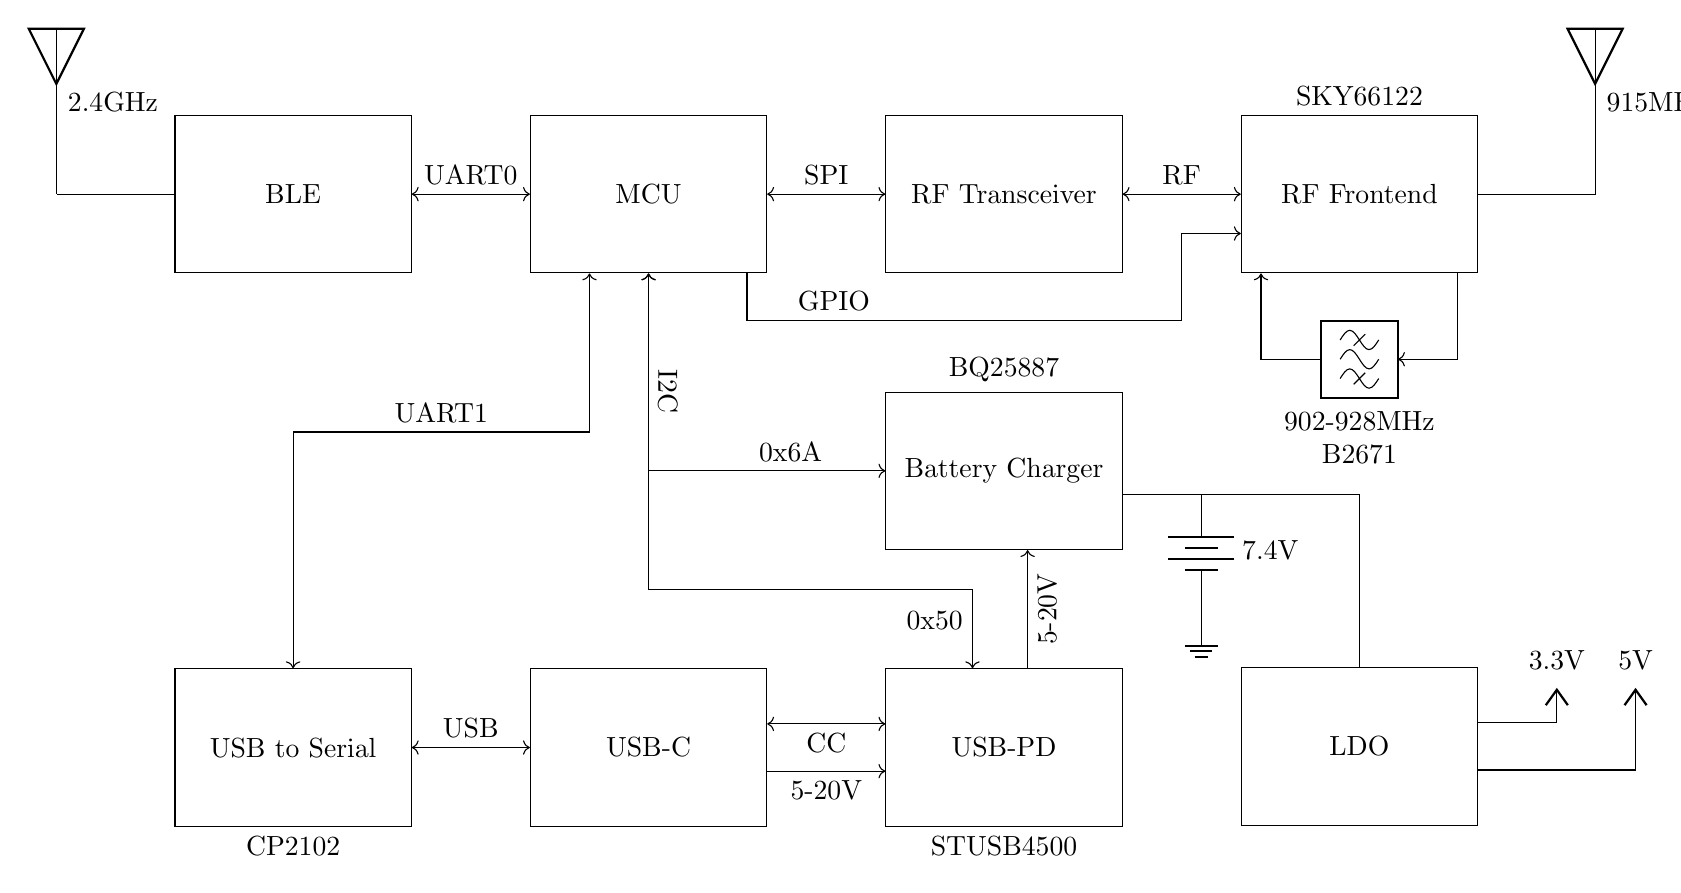
\begin{tikzpicture}[
    block/.style={rectangle, draw, minimum width=2cm, minimum height=1cm},
    io/.style={trapezium, draw, minimum width=2cm},
    arrow/.style={->, thick}
]

% Main MCU Block label=above:{Label text}
\node[block, minimum width=3cm, minimum height=2cm] (mcu) at (0,0) {MCU};
\node[block, right=1.5cm of mcu, minimum width=3cm, minimum height=2cm] (rf) {RF Transceiver};
\node[block, right=1.5cm of rf, minimum width=3cm, minimum height=2cm, label=above:{SKY66122}] (pa) {RF Frontend};
\node[draw, bandpassshape, below=0.6cm of pa, label={[align=center]below:902-928MHz\\B2671}] (bp){};
\node[block, left=1.5cm of mcu, minimum width=3cm, minimum height=2cm] (ble) {BLE};

\node[block, below=1.5cm of rf, minimum width=3cm, minimum height=2cm, label={above:BQ25887}] (chg) {Battery Charger};
\node[block, below=5cm of pa, minimum width=3cm, minimum height=2cm] (ldo) {LDO};
\node[block, below=1.5cm of chg, minimum width=3cm, minimum height=2cm, label={below:STUSB4500}] (usbpd) {USB-PD};
\node[block, left=1.5cm of usbpd, minimum width=3cm, minimum height=2cm] (usbc) {USB-C};
\node[block, left=1.5cm of usbc, minimum width=3cm, minimum height=2cm, label={below:CP2102}] (com) {USB to Serial};

\draw(pa) -- ++(3,0) node[antenna]{915MHz};
\draw(ble) -- ++(-3,0) node[antenna]{2.4GHz};
\draw(mcu)[<->] -- (ble) node[midway, above] {UART0};
\draw(mcu)[<->] -- (rf) node[midway, above] {SPI};
\draw(mcu.south)++(1.25, 0) |- ([xshift=-0.75cm, yshift=-1.6cm] pa.west)node[pos=0.6, above, sloped]{GPIO}[->] |- ([yshift=-0.5cm]pa.west);
\draw (chg.east)++(0,-0.3) -- ++(+1,0)coordinate(bat) to[battery, l=7.4V] ++(0,-1.5) -- ++(0,0) node[ground]{};
\draw(pa.south)++(1.25, 0)[->] |- (bp.east);
\draw(bp.west)[->] -| ([xshift=-1.25cm] pa.south);
\draw(rf)[<->] -- (pa) node[midway, above]{RF};

\draw(usbc)[<->] -- (com) node[midway, above] {USB};
\draw(mcu.south)++(-0.75, 0)[<->] |- ([yshift=3cm]com.north) node [pos=0.75, above, sloped]{UART1} -| (com.north);

\draw(mcu.south)++(0, 0)[<->] |- (chg) node[pos=0.3, above, sloped]{I2C} node[pos=0.8, above]{0x6A};

\draw(mcu.south)++(0, 0)[<->] |- ([yshift=1cm, xshift=-1.0cm]usbpd.north) -| ([xshift=-0.4cm]usbpd.north) node[pos=0.7, left]{0x50};
\draw(usbpd.west)[<->]++(0,0.3) -- ([yshift=0.3cm]usbc.east) node[midway, below]{CC};
\draw(usbpd.west)[<-]++(0,-0.3) -- ([yshift=-0.3cm]usbc.east) node[midway, below]{5-20V};
\draw(usbpd.north)[->]++(0.3,0) -- ([xshift=0.3cm]chg.south) node[midway, below, sloped]{5-20V};
\draw(ldo.north) |- (bat);

\draw(ldo.east)++(0,0.3) -- ++(1,0) node[vcc]{3.3V};
\draw(ldo.east)++(0,-0.3) -| ++(2,0.6) node[vcc]{5V};

\end{tikzpicture}

\end{landscape}





\newpage
\begin{landscape}
\section*{Component Selection Option A (STM32)}
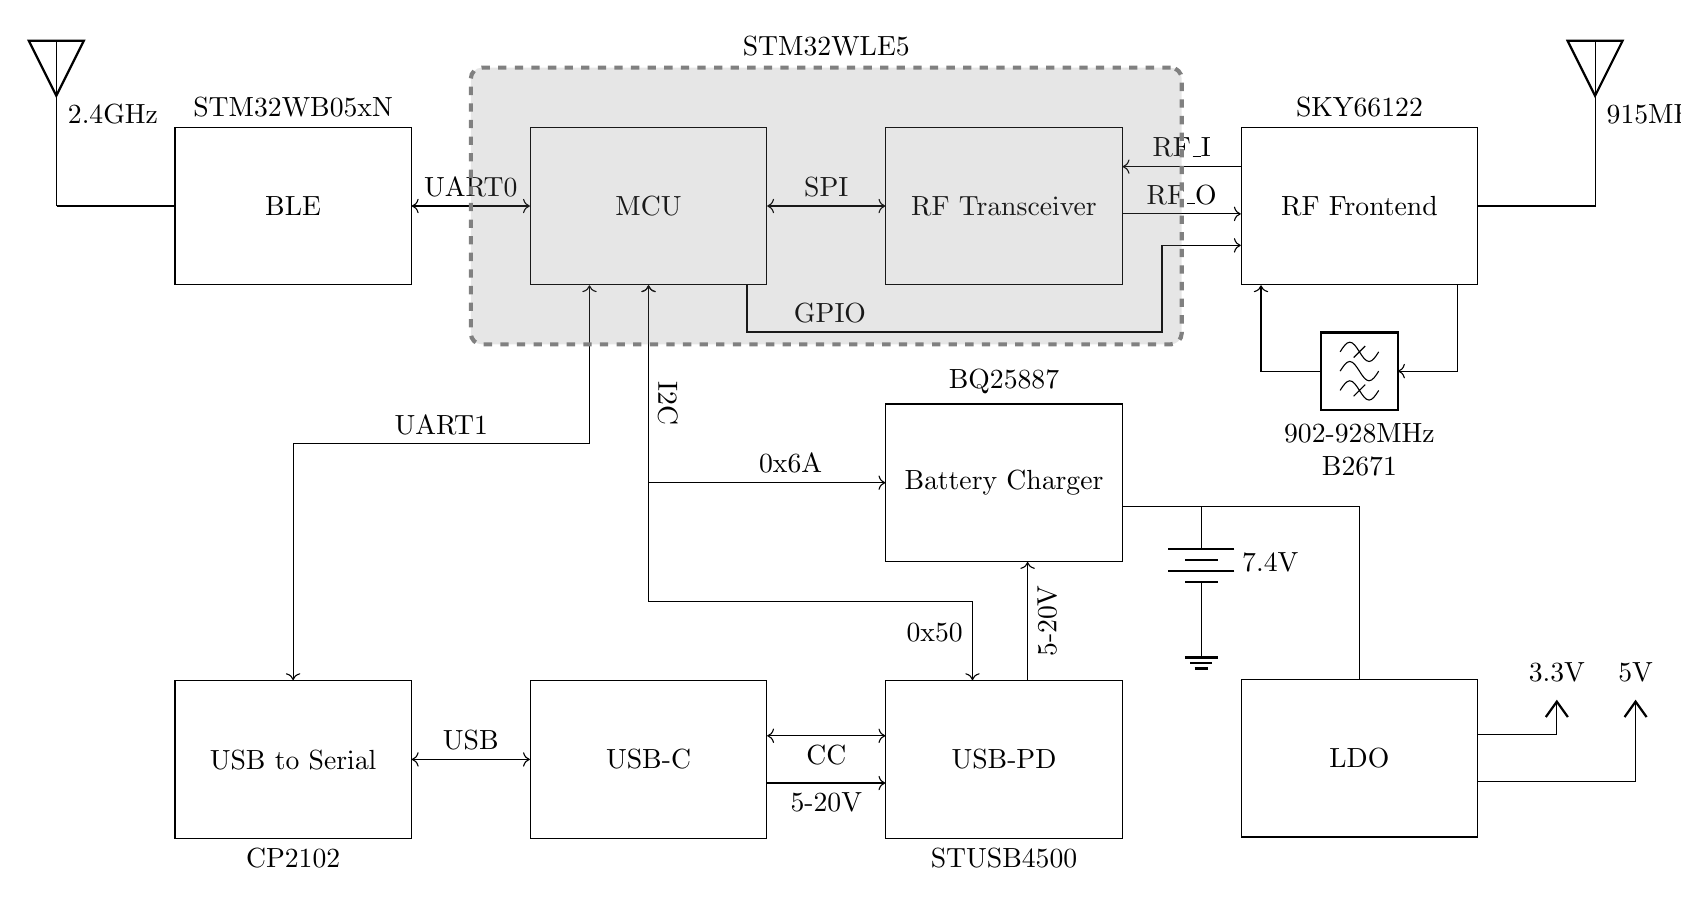
\begin{tikzpicture}[
    block/.style={rectangle, draw, minimum width=2cm, minimum height=1cm},
    io/.style={trapezium, draw, minimum width=2cm},
    arrow/.style={->, thick}
]

% Main MCU Block label=above:{Label text}
\node[block, minimum width=3cm, minimum height=2cm] (mcu) at (0,0) {MCU};
\node[block, right=1.5cm of mcu, minimum width=3cm, minimum height=2cm] (rf) {RF Transceiver};
\node[block, right=1.5cm of rf, minimum width=3cm, minimum height=2cm, label=above:{SKY66122}] (pa) {RF Frontend};
\node[draw, bandpassshape, below=0.6cm of pa, label={[align=center]below:902-928MHz\\B2671}] (bp){};
\node[block, left=1.5cm of mcu, minimum width=3cm, minimum height=2cm, label={above:STM32WB05xN}] (ble) {BLE};

\node[block, below=1.5cm of rf, minimum width=3cm, minimum height=2cm, label={above:BQ25887}] (chg) {Battery Charger};
\node[block, below=5cm of pa, minimum width=3cm, minimum height=2cm] (ldo) {LDO};
\node[block, below=1.5cm of chg, minimum width=3cm, minimum height=2cm, label={below:STUSB4500}] (usbpd) {USB-PD};
\node[block, left=1.5cm of usbpd, minimum width=3cm, minimum height=2cm] (usbc) {USB-C};
\node[block, left=1.5cm of usbc, minimum width=3cm, minimum height=2cm, label={below:CP2102}] (com) {USB to Serial};

\draw(pa) -- ++(3,0) node[antenna]{915MHz};
\draw(ble) -- ++(-3,0) node[antenna]{2.4GHz};
\draw(mcu)[<->] -- (ble) node[midway, above] {UART0};
\draw(mcu)[<->] -- (rf) node[midway, above] {SPI};
\draw(mcu.south)++(1.25, 0) |- ([xshift=-1cm, yshift=-1.6cm] pa.west)node[pos=0.6, above, sloped]{GPIO}[->] |- ([yshift=-0.5cm]pa.west);
\draw (chg.east)++(0,-0.3) -- ++(+1,0)coordinate(bat) to[battery, l=7.4V] ++(0,-1.5) -- ++(0,0) node[ground]{};
\draw(pa.south)++(1.25, 0)[->] |- (bp.east);
\draw(bp.west)[->] -| ([xshift=-1.25cm] pa.south);
\draw(rf.east)[<-]++(0, 0.5) -- ([yshift=0.5cm]pa.west) node[midway, above]{RF\_I};
\draw(rf.east)[->]++(0, -0.1) -- ([yshift=-0.1cm]pa.west) node[midway, above]{RF\_O};

\draw(usbc)[<->] -- (com) node[midway, above] {USB};
\draw(mcu.south)++(-0.75, 0)[<->] |- ([yshift=3cm]com.north) node [pos=0.75, above, sloped]{UART1} -| (com.north);

\draw(mcu.south)++(0, 0)[<->] |- (chg) node[pos=0.3, above, sloped]{I2C} node[pos=0.8, above]{0x6A};

\draw(mcu.south)++(0, 0)[<->] |- ([yshift=1cm, xshift=-1.0cm]usbpd.north) -| ([xshift=-0.4cm]usbpd.north) node[pos=0.7, left]{0x50};
\draw(usbpd.west)[<->]++(0,0.3) -- ([yshift=0.3cm]usbc.east) node[midway, below]{CC};
\draw(usbpd.west)[<-]++(0,-0.3) -- ([yshift=-0.3cm]usbc.east) node[midway, below]{5-20V};
\draw(usbpd.north)[->]++(0.3,0) -- ([xshift=0.3cm]chg.south) node[midway, below, sloped]{5-20V};
\draw(ldo.north) |- (bat);

\draw(ldo.east)++(0,0.3) -- ++(1,0) node[vcc]{3.3V};
\draw(ldo.east)++(0,-0.3) -| ++(2,0.6) node[vcc]{5V};

\node[draw, dashed, gray, line width=1.5pt, fill=gray, fill opacity = 0.2, rounded corners, fit=(mcu) (rf), inner sep=0.75cm, label={above:STM32WLE5}] {};

\end{tikzpicture}

\end{landscape}




\newpage
\begin{landscape}
\section*{Component Selection Option B (nRF52840)}
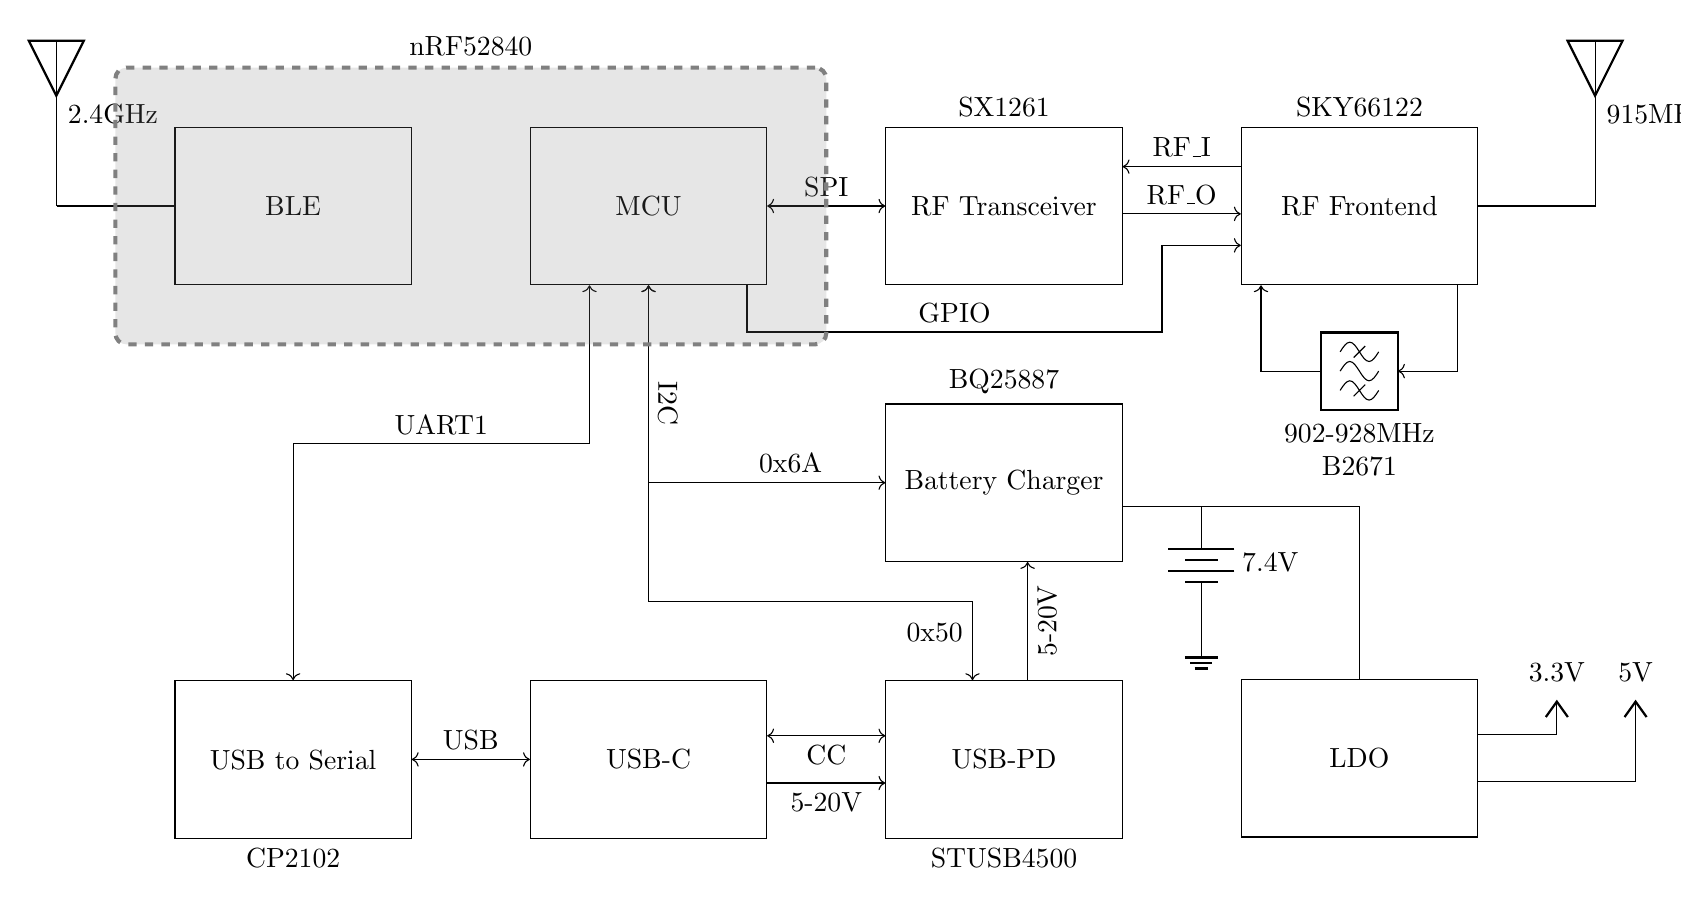
\begin{tikzpicture}[
    block/.style={rectangle, draw, minimum width=2cm, minimum height=1cm},
    io/.style={trapezium, draw, minimum width=2cm},
    arrow/.style={->, thick}
]

% Main MCU Block label=above:{Label text}
\node[block, minimum width=3cm, minimum height=2cm] (mcu) at (0,0) {MCU};
\node[block, right=1.5cm of mcu, minimum width=3cm, minimum height=2cm, label={above:SX1261}] (rf) {RF Transceiver};
\node[block, right=1.5cm of rf, minimum width=3cm, minimum height=2cm, label=above:{SKY66122}] (pa) {RF Frontend};
\node[draw, bandpassshape, below=0.6cm of pa, label={[align=center]below:902-928MHz\\B2671}] (bp){};
\node[block, left=1.5cm of mcu, minimum width=3cm, minimum height=2cm] (ble) {BLE};

\node[block, below=1.5cm of rf, minimum width=3cm, minimum height=2cm, label={above:BQ25887}] (chg) {Battery Charger};
\node[block, below=5cm of pa, minimum width=3cm, minimum height=2cm] (ldo) {LDO};
\node[block, below=1.5cm of chg, minimum width=3cm, minimum height=2cm, label={below:STUSB4500}] (usbpd) {USB-PD};
\node[block, left=1.5cm of usbpd, minimum width=3cm, minimum height=2cm] (usbc) {USB-C};
\node[block, left=1.5cm of usbc, minimum width=3cm, minimum height=2cm, label={below:CP2102}] (com) {USB to Serial};

\draw(pa) -- ++(3,0) node[antenna]{915MHz};
\draw(ble) -- ++(-3,0) node[antenna]{2.4GHz};
\draw(mcu)[<->] -- (rf) node[midway, above] {SPI};
\draw(mcu.south)++(1.25, 0) |- ([xshift=-1cm, yshift=-1.6cm] pa.west)node[pos=0.75, above, sloped]{GPIO}[->] |- ([yshift=-0.5cm]pa.west);
\draw (chg.east)++(0,-0.3) -- ++(+1,0)coordinate(bat) to[battery, l=7.4V] ++(0,-1.5) -- ++(0,0) node[ground]{};
\draw(pa.south)++(1.25, 0)[->] |- (bp.east);
\draw(bp.west)[->] -| ([xshift=-1.25cm] pa.south);
\draw(rf.east)[<-]++(0, 0.5) -- ([yshift=0.5cm]pa.west) node[midway, above]{RF\_I};
\draw(rf.east)[->]++(0, -0.1) -- ([yshift=-0.1cm]pa.west) node[midway, above]{RF\_O};

\draw(usbc)[<->] -- (com) node[midway, above] {USB};
\draw(mcu.south)++(-0.75, 0)[<->] |- ([yshift=3cm]com.north) node [pos=0.75, above, sloped]{UART1} -| (com.north);

\draw(mcu.south)++(0, 0)[<->] |- (chg) node[pos=0.3, above, sloped]{I2C} node[pos=0.8, above]{0x6A};

\draw(mcu.south)++(0, 0)[<->] |- ([yshift=1cm, xshift=-1.0cm]usbpd.north) -| ([xshift=-0.4cm]usbpd.north) node[pos=0.7, left]{0x50};
\draw(usbpd.west)[<->]++(0,0.3) -- ([yshift=0.3cm]usbc.east) node[midway, below]{CC};
\draw(usbpd.west)[<-]++(0,-0.3) -- ([yshift=-0.3cm]usbc.east) node[midway, below]{5-20V};
\draw(usbpd.north)[->]++(0.3,0) -- ([xshift=0.3cm]chg.south) node[midway, below, sloped]{5-20V};
\draw(ldo.north) |- (bat);

\draw(ldo.east)++(0,0.3) -- ++(1,0) node[vcc]{3.3V};
\draw(ldo.east)++(0,-0.3) -| ++(2,0.6) node[vcc]{5V};

\node[draw, dashed, gray, line width=1.5pt, fill=gray, fill opacity = 0.2, rounded corners, fit=(mcu) (ble), inner sep=0.75cm, label={above:nRF52840}] {};

\end{tikzpicture}

\end{landscape}







\newpage
\begin{landscape}
\section*{Component Selection Option C-1 (ESP32C3)}
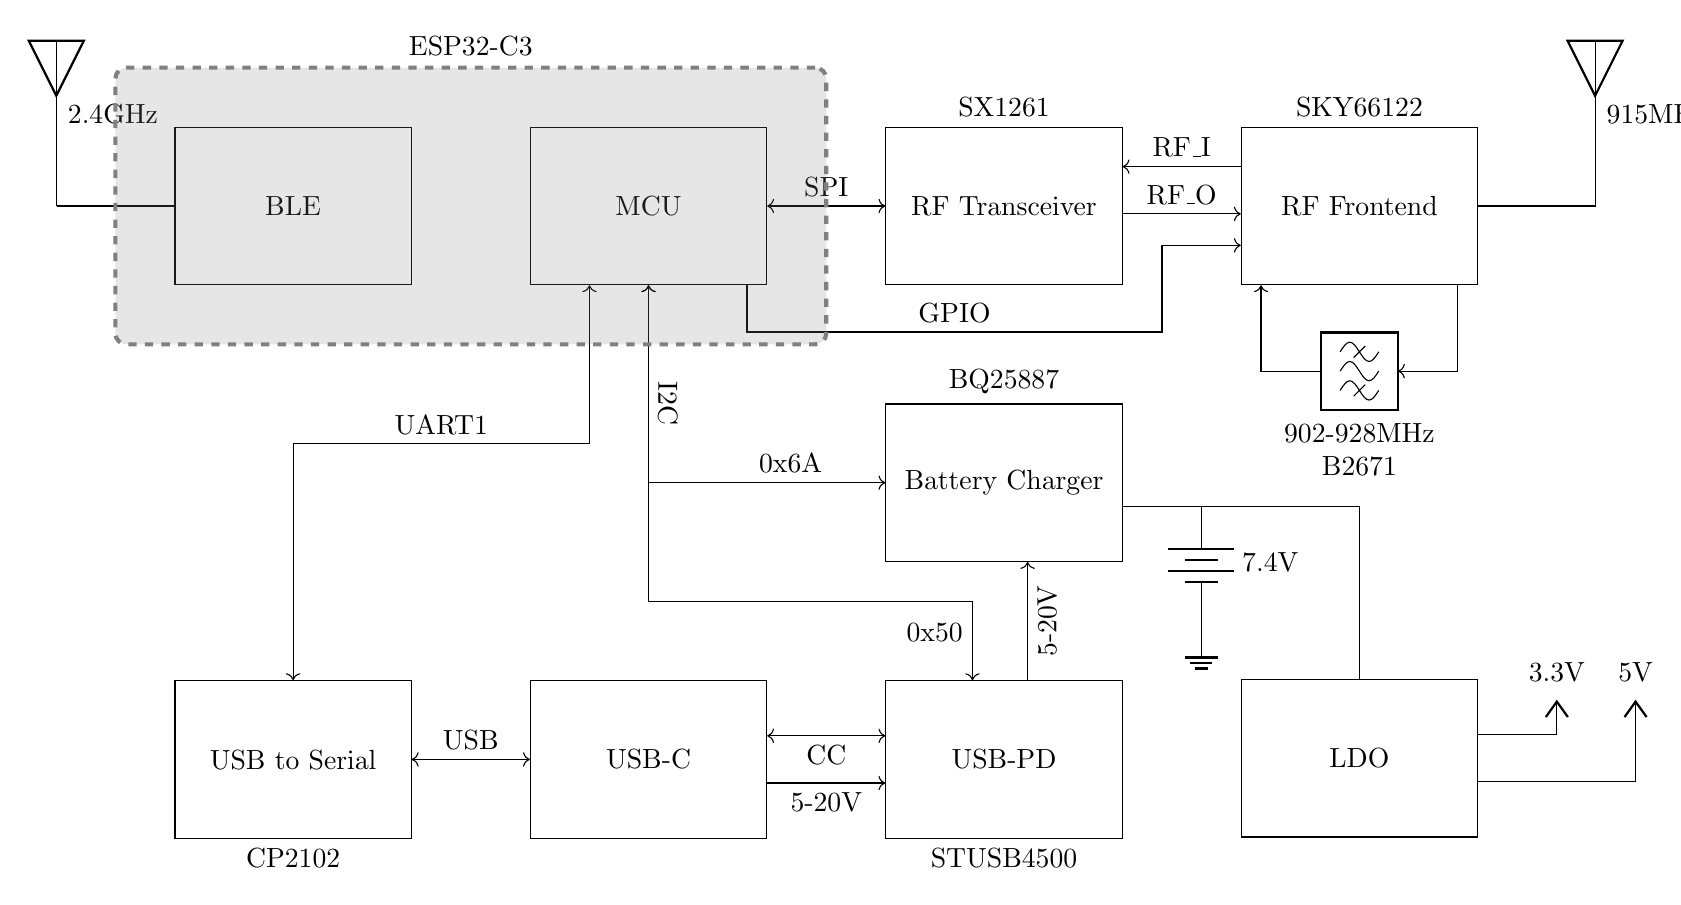
\begin{tikzpicture}[
    block/.style={rectangle, draw, minimum width=2cm, minimum height=1cm},
    io/.style={trapezium, draw, minimum width=2cm},
    arrow/.style={->, thick}
]

% Main MCU Block label=above:{Label text}
\node[block, minimum width=3cm, minimum height=2cm] (mcu) at (0,0) {MCU};
\node[block, right=1.5cm of mcu, minimum width=3cm, minimum height=2cm, label={above:SX1261}] (rf) {RF Transceiver};
\node[block, right=1.5cm of rf, minimum width=3cm, minimum height=2cm, label=above:{SKY66122}] (pa) {RF Frontend};
\node[draw, bandpassshape, below=0.6cm of pa, label={[align=center]below:902-928MHz\\B2671}] (bp){};
\node[block, left=1.5cm of mcu, minimum width=3cm, minimum height=2cm] (ble) {BLE};

\node[block, below=1.5cm of rf, minimum width=3cm, minimum height=2cm, label={above:BQ25887}] (chg) {Battery Charger};
\node[block, below=5cm of pa, minimum width=3cm, minimum height=2cm] (ldo) {LDO};
\node[block, below=1.5cm of chg, minimum width=3cm, minimum height=2cm, label={below:STUSB4500}] (usbpd) {USB-PD};
\node[block, left=1.5cm of usbpd, minimum width=3cm, minimum height=2cm] (usbc) {USB-C};
\node[block, left=1.5cm of usbc, minimum width=3cm, minimum height=2cm, label={below:CP2102}] (com) {USB to Serial};

\draw(pa) -- ++(3,0) node[antenna]{915MHz};
\draw(ble) -- ++(-3,0) node[antenna]{2.4GHz};
\draw(mcu)[<->] -- (rf) node[midway, above] {SPI};
\draw(mcu.south)++(1.25, 0) |- ([xshift=-1cm, yshift=-1.6cm] pa.west)node[pos=0.75, above, sloped]{GPIO}[->] |- ([yshift=-0.5cm]pa.west);
\draw (chg.east)++(0,-0.3) -- ++(+1,0)coordinate(bat) to[battery, l=7.4V] ++(0,-1.5) -- ++(0,0) node[ground]{};
\draw(pa.south)++(1.25, 0)[->] |- (bp.east);
\draw(bp.west)[->] -| ([xshift=-1.25cm] pa.south);
\draw(rf.east)[<-]++(0, 0.5) -- ([yshift=0.5cm]pa.west) node[midway, above]{RF\_I};
\draw(rf.east)[->]++(0, -0.1) -- ([yshift=-0.1cm]pa.west) node[midway, above]{RF\_O};

\draw(usbc)[<->] -- (com) node[midway, above] {USB};
\draw(mcu.south)++(-0.75, 0)[<->] |- ([yshift=3cm]com.north) node [pos=0.75, above, sloped]{UART1} -| (com.north);

\draw(mcu.south)++(0, 0)[<->] |- (chg) node[pos=0.3, above, sloped]{I2C} node[pos=0.8, above]{0x6A};

\draw(mcu.south)++(0, 0)[<->] |- ([yshift=1cm, xshift=-1.0cm]usbpd.north) -| ([xshift=-0.4cm]usbpd.north) node[pos=0.7, left]{0x50};
\draw(usbpd.west)[<->]++(0,0.3) -- ([yshift=0.3cm]usbc.east) node[midway, below]{CC};
\draw(usbpd.west)[<-]++(0,-0.3) -- ([yshift=-0.3cm]usbc.east) node[midway, below]{5-20V};
\draw(usbpd.north)[->]++(0.3,0) -- ([xshift=0.3cm]chg.south) node[midway, below, sloped]{5-20V};
\draw(ldo.north) |- (bat);

\draw(ldo.east)++(0,0.3) -- ++(1,0) node[vcc]{3.3V};
\draw(ldo.east)++(0,-0.3) -| ++(2,0.6) node[vcc]{5V};

\node[draw, dashed, gray, line width=1.5pt, fill=gray, fill opacity = 0.2, rounded corners, fit=(mcu) (ble), inner sep=0.75cm, label={above:ESP32-C3}] {};

\end{tikzpicture}

\end{landscape}




\newpage
\begin{landscape}
\section*{Component Selection Option C-2 (ESP32S3)}
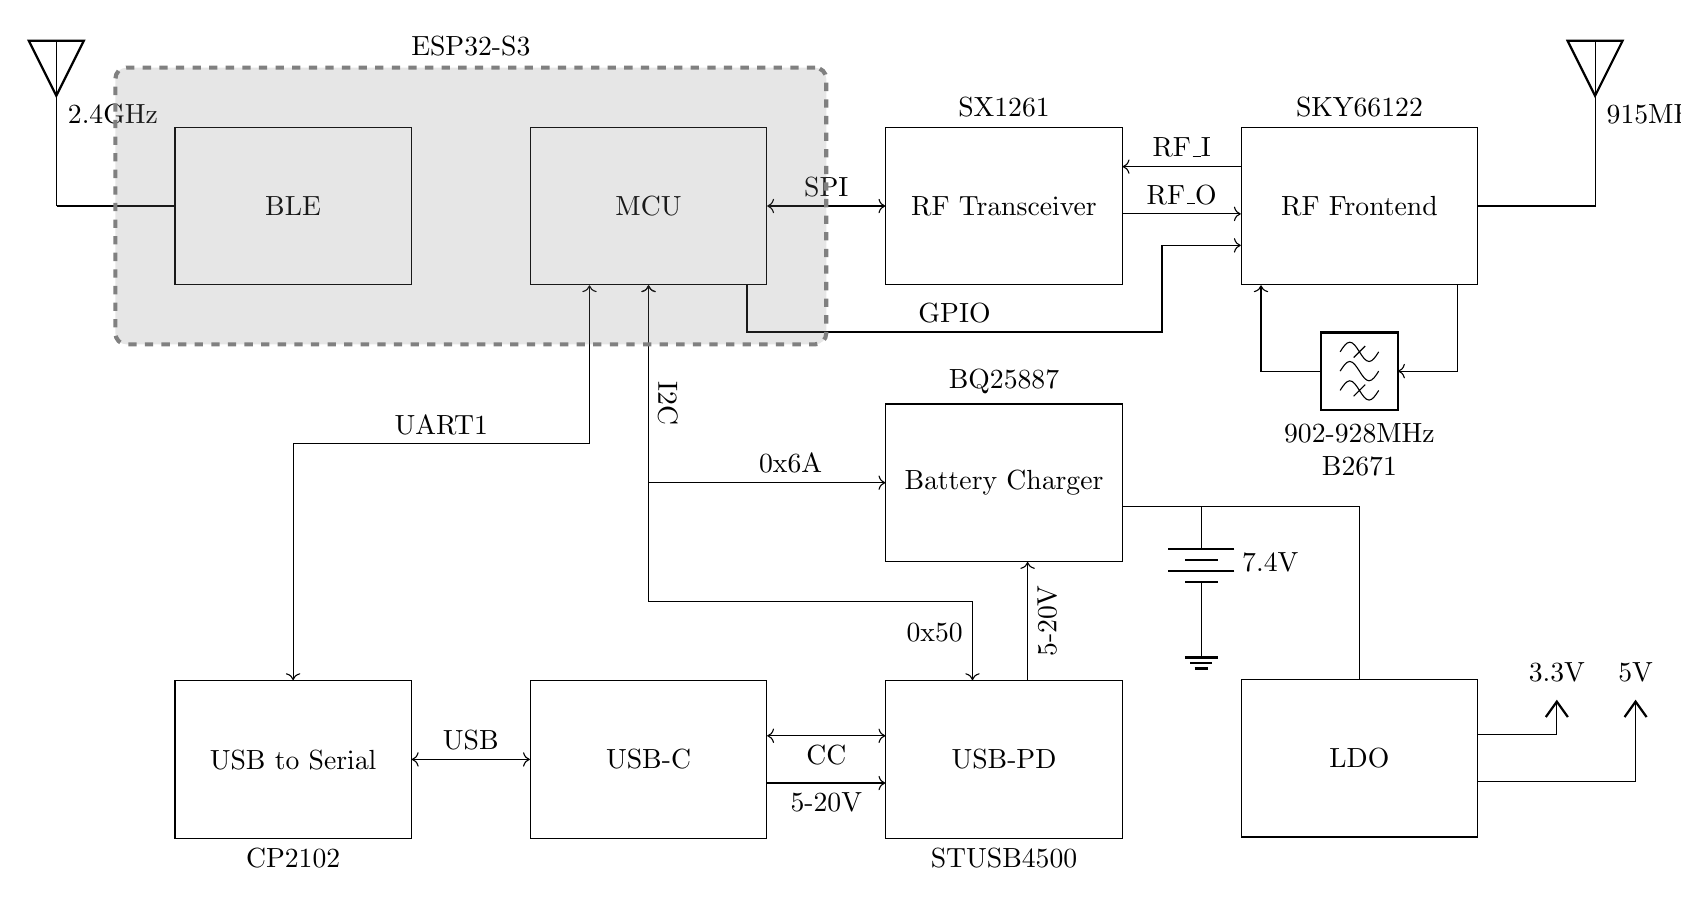
\begin{tikzpicture}[
    block/.style={rectangle, draw, minimum width=2cm, minimum height=1cm},
    io/.style={trapezium, draw, minimum width=2cm},
    arrow/.style={->, thick}
]

% Main MCU Block label=above:{Label text}
\node[block, minimum width=3cm, minimum height=2cm] (mcu) at (0,0) {MCU};
\node[block, right=1.5cm of mcu, minimum width=3cm, minimum height=2cm, label={above:SX1261}] (rf) {RF Transceiver};
\node[block, right=1.5cm of rf, minimum width=3cm, minimum height=2cm, label=above:{SKY66122}] (pa) {RF Frontend};
\node[draw, bandpassshape, below=0.6cm of pa, label={[align=center]below:902-928MHz\\B2671}] (bp){};
\node[block, left=1.5cm of mcu, minimum width=3cm, minimum height=2cm] (ble) {BLE};

\node[block, below=1.5cm of rf, minimum width=3cm, minimum height=2cm, label={above:BQ25887}] (chg) {Battery Charger};
\node[block, below=5cm of pa, minimum width=3cm, minimum height=2cm] (ldo) {LDO};
\node[block, below=1.5cm of chg, minimum width=3cm, minimum height=2cm, label={below:STUSB4500}] (usbpd) {USB-PD};
\node[block, left=1.5cm of usbpd, minimum width=3cm, minimum height=2cm] (usbc) {USB-C};
\node[block, left=1.5cm of usbc, minimum width=3cm, minimum height=2cm, label={below:CP2102}] (com) {USB to Serial};

\draw(pa) -- ++(3,0) node[antenna]{915MHz};
\draw(ble) -- ++(-3,0) node[antenna]{2.4GHz};
\draw(mcu)[<->] -- (rf) node[midway, above] {SPI};
\draw(mcu.south)++(1.25, 0) |- ([xshift=-1cm, yshift=-1.6cm] pa.west)node[pos=0.75, above, sloped]{GPIO}[->] |- ([yshift=-0.5cm]pa.west);
\draw (chg.east)++(0,-0.3) -- ++(+1,0)coordinate(bat) to[battery, l=7.4V] ++(0,-1.5) -- ++(0,0) node[ground]{};
\draw(pa.south)++(1.25, 0)[->] |- (bp.east);
\draw(bp.west)[->] -| ([xshift=-1.25cm] pa.south);
\draw(rf.east)[<-]++(0, 0.5) -- ([yshift=0.5cm]pa.west) node[midway, above]{RF\_I};
\draw(rf.east)[->]++(0, -0.1) -- ([yshift=-0.1cm]pa.west) node[midway, above]{RF\_O};

\draw(usbc)[<->] -- (com) node[midway, above] {USB};
\draw(mcu.south)++(-0.75, 0)[<->] |- ([yshift=3cm]com.north) node [pos=0.75, above, sloped]{UART1} -| (com.north);

\draw(mcu.south)++(0, 0)[<->] |- (chg) node[pos=0.3, above, sloped]{I2C} node[pos=0.8, above]{0x6A};

\draw(mcu.south)++(0, 0)[<->] |- ([yshift=1cm, xshift=-1.0cm]usbpd.north) -| ([xshift=-0.4cm]usbpd.north) node[pos=0.7, left]{0x50};
\draw(usbpd.west)[<->]++(0,0.3) -- ([yshift=0.3cm]usbc.east) node[midway, below]{CC};
\draw(usbpd.west)[<-]++(0,-0.3) -- ([yshift=-0.3cm]usbc.east) node[midway, below]{5-20V};
\draw(usbpd.north)[->]++(0.3,0) -- ([xshift=0.3cm]chg.south) node[midway, below, sloped]{5-20V};
\draw(ldo.north) |- (bat);

\draw(ldo.east)++(0,0.3) -- ++(1,0) node[vcc]{3.3V};
\draw(ldo.east)++(0,-0.3) -| ++(2,0.6) node[vcc]{5V};

\node[draw, dashed, gray, line width=1.5pt, fill=gray, fill opacity = 0.2, rounded corners, fit=(mcu) (ble), inner sep=0.75cm, label={above:ESP32-S3}] {};

\end{tikzpicture}

\end{landscape}





\newpage
\section{Power Consumption Analysis}
\subsection{Component Current Requirements}

\begin{table}[h]
\centering
\caption*{Option A}
\begin{tabular}{|l|c|c|c|}
\hline
\textbf{Component} & \textbf{Part Number} & \textbf{Peak Current (mA)} & \textbf{Continuous Current (mA)} \\
\hline
BLE & STM32WB05xN & 100 & 25 \\
\hline
MCU & \multirow{2}{*}{STM32WLE5} & 100 & 25 \\
\cline{1-1}\cline{3-4}
RF Transceiver &   & 95 & 15 \\
\hline
RF Frontend & SKY66122 & 500 & 50 \\
\hline
Battery Charger & BQ25887 & 200 & 5 \\
\hline
USB-PD & STUSB4500 & 30 & 8 \\
\hline
USB-C & Generic & 10 & 2 \\
\hline
USB to Serial & CP2102 & 80 & 20 \\
\Xhline{5\arrayrulewidth}
\multicolumn{2}{|c|}{\textbf{Total}} & \textbf{150 mA} &  \textbf{150 mA} \\
\hline

\end{tabular}
\end{table}

\newpage
\section{LDO Selection}


\end{document}